\chapter{\LaTeX-Beispiele}
	\emph{Dieses Kapitel beinhaltet Beispiele und kurze Erklärungen zu verschiedenen \LaTeX-Funktionen die in einer wissenschaftlichen Ausarbeitung nützlich sein könnten.%
%	Wie diese konkret benutzt werden, kann man im \LaTeX-Quellcode der Thesisvorlage %(Datei \lstinline|LaTeX-Beispiele.tex|)
%	 sehen.
	 }
		
	\section{Kapitel, Abschnitte, Paragraphen}\label{sec:chapter-section-paragraph}
		Kapitel werden mit \lstinline|\chapter{Kapitelname}| erstellt.
		Als nächste Ebenen folgen \lstinline|\section{title}|, \lstinline|\subsection{title}| und \lstinline|\subsubsection{title}|.
		Reicht das immer noch nicht, gibt es auch noch \lstinline|\paragraph{title}| und für den aller äußersten Notfall\footnote{Wer so viele Hierarchieebenen benötigt mach in der Regel etwas falsch -- Selbst außergewöhnlich lange Bachelor- und Master-Thesen sind normalerweise nicht so umfangreich, dass Subparagraphen nötig werden} sogar noch \lstinline|\subparagraph{title}|.
		\begin{vorlagenbeispiel}
			\subsection{Subsection}
				Hier sind wir in einer Subsection.
				\subsubsection{Subsubsection}
					Hier sind wir in einer Subsubsection.
					\paragraph{Paragraph}
						Hier sind wir in einem Paragraph.
%						\subparagraph{Subparagraph}
%							Hier sind wir in einem Subparagraph.
		\end{vorlagenbeispiel}
		
	\section{Textauszeichnung}
		\begin{vorlagenbeispiel}
			Text kann man zum Beispiel \textbf{Fett}, \textit{Kursiv} oder \underline{Unterstrichen} hervorheben. Das geht aber auch mit \textsc{Kapitälchen}, \texttt{Dicktengleicher Schrift} oder \textsf{Serifenloser Schrift}.
		\end{vorlagenbeispiel}
		\begin{lstlisting}[keywords={textbf, textit, underline, textsc, texttt, textsf}]
Text kann man zum Beispiel \textbf{Fett}, \textit{Kursiv} oder \underline{Unterstrichen} hervorheben. Das geht aber auch mit \textsc{Kapitälchen}, \texttt{Dicktengleicher Schrift} oder \textsf{Serifenloser Schrift}.
		\end{lstlisting}
					
	\section{Fußnoten}
		\begin{vorlagenbeispiel}
		Ein Text kann Fußnoten\footnote{Wie z.B. diese hier} enthalten.
		\end{vorlagenbeispiel}
		Diese werden mit \lstinline|\footnote{text}| gesetzt. Formatierungen in der Fußnote sind grundsätzlich kein Problem%
		\footnote{%
			\color{red}Dies ist eine besonders \textbf{fette Fußnote} in rot.
		}.
%		
		Aber Vorsicht: Manche Befehle wie \zb \lstinline|\lstinline| können nicht ohne weiteres/nicht immer in einer Fußnote gesetzt werden\footnote{Der Grund dafür lässt sich unter \url{https://www.texfaq.org/FAQ-verbwithin} nachlesen}.
	
	\section{Zitate \& Literaturangaben}
		\subsection{Zitieren}
			Korrektes Zitieren ist in der Wissenschaft \emph{(und auch sonst)} äußerst wichtig und daher Pflicht.
%			\medskip
%			
			Bei allem%
				\footnote{Basiswissen aus dem jeweiligen Fachbereich muss in der Regel nicht zitiert werden, d.h. ein Student der Elektotechnik muss $U = R \cdot I$ nicht zitieren, ein Kunststudent, der ein paar LEDs anschließen möchte und dafür einen Vorwiderstand berechnet, ansonsten aber noch nie etwas von dieser Formel gehört hat, sollte dies hingegen schon.}%
			, was man von anderen übernommen hat, muss angegeben werden, woher es stammt und wer es verfasst/veröffentlicht hat.
				\medskip
					
			Auf diese Weise wird eindeutig gezeigt, dass eine Information aus einer anderen Quelle übernommen wurde.
			Übernimmt man Informationen, lässt aber den Quellenverweis weg, suggeriert man damit fälschlicherweise man sei selbst die Quelle.
			\textbf{%
				Dies macht die entsprechende Stelle dann zu einem Plagiat} -- in der Regel ein vernichtendes Urteil für jede Arbeit und normalerweise ein schneller Weg bei Thesis, Praktikum, Seminar \& co. in Schimpf und Schande durchzufallen!
%			}
			\medskip
		
			\emph{\paragraph{Aber keine Panik...}
				Wer grundsätzlich gewissenhaft zitiert, an einer Stelle aber mal eine Zitierklammer vergisst, fällt damit natürlich nicht direkt durch...}
				
				
		\subsection{Literaturverzeichnis}
			Literatur wird in der Datei \lstinline|Literatur.bib| angegeben und in der Thesis dann mit dem Befehl \lstinline[language=thesis-latexbeispiel]|\cite{literaturname}| zitiert\cite{thesis:vorlage}.
			\medskip
			
			Am einfachsten ist die Bearbeitung der Datei \lstinline|Literatur.bib| mit einem Literaturverwaltungsprogramm wie beispielsweise dem frei verfügbaren \href{https://www.jabref.org/}{\emph{JabRef}}
		
		\subsection{Zitate in \LaTeX}
			Zitieren kann man auf viele Arten.
			Dabei reicht es aber nicht, den Text einfach nur in Anführungszeichen zu setzen, z.\,B. \enquote{Text}!
			Für ein korrektes Zitat muss immer auch die Quellenangabe erkennbar sein.
			Dabei kann in einem Satz, der etwas behauptet, direkt die Zitierklammer gesetzt werden:
			\begin{vorlagenbeispiel}
				Der AXI-Bus hat dabei eine Datenbreite, die stets ein Vielfaches von acht Bit\cite{ARM:AMBA4AXI4StreamProtocol:v1_0} ist.
			\end{vorlagenbeispiel}
			\begin{lstlisting}[language=thesis-latexbeispiel, numbers=none]
Der AXI-Bus hat dabei eine Datenbreite, die stets ein Vielfaches von acht Bit\cite{ARM:AMBA4AXI4StreamProtocol:v1_0} ist.
			\end{lstlisting}
			
			So richtig hilfreich wird ein Zitat natürlich erst, wenn wir dem Leser auch einen Hinweis geben, an welcher Stelle (also \zb{} in welchem Kapitel oder auf welcher Seite) er in der angegebenen Quelle suchen muss:
			\begin{vorlagenbeispiel}
				Der AXI-Bus hat dabei eine Datenbreite, die stets ein Vielfaches von acht Bit\cite[S.42]{ARM:AMBA4AXI4StreamProtocol:v1_0} ist.
			\end{vorlagenbeispiel}
			\begin{lstlisting}[language=thesis-latexbeispiel, numbers=none]
Der AXI-Bus hat dabei eine Datenbreite, die stets ein Vielfaches von acht Bit\cite[S.42]{ARM:AMBA4AXI4StreamProtocol:v1_0} ist.
			\end{lstlisting}
			\medskip
			
			\noindent
			Zitat in einer anderen Sprache:
			\begin{vorlagenbeispiel}
				\foreignquote{english}{An apple a day keeps the doctor away.}
			\end{vorlagenbeispiel}
			\begin{lstlisting}[language=thesis-latexbeispiel, numbers=none]
\foreignquote{english}{An apple a day keeps the doctor away.}
			\end{lstlisting}
			\medskip
			
			\noindent
			Wörtliches Zitat direkt mit Quelle: 
			\begin{vorlagenbeispiel}
				\textquote[{\cite[\thepage]{thesis:vorlage}}]{Hier steht der Zitat-Text}
			\end{vorlagenbeispiel}
			\begin{lstlisting}[language=thesis-latexbeispiel, numbers=none, escapeinside={*}{*}]
\textquote[{\cite[*\thepage*]{ARM:NEONProgrammersGuide:v1_0}}][.]{Hier steht der Zitat-Text}
			\end{lstlisting}
			\medskip
		
			\noindent
			Blockzitat: Ab einer bestimmten Länge wird das Zitat wie hier gezeigt als eingerückter Block dargestellt:
%			
			\begin{vorlagenbeispiel}
				\blockquote[{\cite[\thepage]{thesis:vorlage}}]{%
					Hier steht der Zitat-Text. Hier steht der Zitat-Text.Hier steht der Zitat-Text.Hier steht der Zitat-Text.Hier steht der Zitat-Text.Hier steht der Zitat-Text.Hier steht der Zitat-Text.Hier steht der Zitat-Text.Hier steht der Zitat-Text.Hier steht der Zitat-Text.Hier steht der Zitat-Text.Hier steht der Zitat-Text.Hier steht der Zitat-Text.Hier steht der Zitat-Text.Hier steht der Zitat-Text.Hier steht der Zitat-Text.Hier steht der Zitat-Text.Hier steht der Zitat-Text.Hier steht der Zitat-Text.Hier steht der Zitat-Text.Hier steht der Zitat-Text.Hier steht der Zitat-Text.Hier steht der Zitat-Text.Hier steht der Zitat-Text.Hier steht der Zitat-Text.
				}
			\end{vorlagenbeispiel}
			\begin{lstlisting}[language=thesis-latexbeispiel, escapeinside={*}{*}]
\blockquote[{\cite[*\thepage*]{thesis:vorlage}}]{%
	Hier steht der Zitat-Text. Hier steht der Zitat-Text.Hier steht der Zitat-Text.Hier steht der Zitat-Text.Hier steht der Zitat-Text.Hier steht der Zitat-Text.Hier steht der Zitat-Text.Hier steht der Zitat-Text.Hier steht der Zitat-Text.Hier steht der Zitat-Text.Hier steht der Zitat-Text.Hier steht der Zitat-Text.Hier steht der Zitat-Text.Hier steht der Zitat-Text.Hier steht der Zitat-Text.Hier steht der Zitat-Text.Hier steht der Zitat-Text.Hier steht der Zitat-Text.Hier steht der Zitat-Text.Hier steht der Zitat-Text.Hier steht der Zitat-Text.Hier steht der Zitat-Text.Hier steht der Zitat-Text.Hier steht der Zitat-Text.Hier steht der Zitat-Text.
}
			\end{lstlisting}
		
	\section{Zahlen und Formeln}
		\subsection{Zahlen-/Einheitendarstellung}
			\emph{Diese Thesisvorlage benutzt das \LaTeX-Paket \lstinline|siunitx|, welches die Darstellung von Zahlen und Einheiten vereinheitlicht. Die gesetzten Paketeinstellungen finden sich in der Konfigurationsdatei \lstinline|siunitx.cfg|}.
			
			\subsubsection{Zahlen}
				Zahlen werden mit \lstinline|\num{3.14159}| gesetzt.
				Verwendet man sehr große/sehr klein Zahlen, so wird dabei automatisch der passende Skalierungsfaktor in der ingenieurstypischen $10^{3x}$-Notation erzeugt.
	%			
				\begin{vorlagenbeispiel}
					So wird etwa \lstinline|\num{4210234}| als \num{4210234} gesetzt und \lstinline|\num{0.00000000002535}| wird zu \num{0.00000000002535}.
				\end{vorlagenbeispiel}
				\medskip
				
				\noindent\fbox{\parbox{0.98\linewidth}{%
					\textbf{Warum nicht direkt schreiben?}
					\itshape\\
					Diese Frage drängt sich geradezu auf: Warum sollte die Zahl nicht einfach so hinschreiben?
					\normalfont\\
					Erstens sorgt die Verwendung der passenden Befehle dafür, dass die Zahlen immer gleich (und typographisch korrekt) formatiert werden und zweitens lässt sich diese Darstellung global, also für das ganze Dokument ändern.
					Weiterhin kümmert sich der Befehl wie gezeigt (wenn passend vorkonfiguriert, dies ist in dieser Vorlage der Fall) automatisch um die Darstellung in den ingenieurstypischen Zehnerpotenzen.
				}}
	
			\subsubsection{Einheiten}
				Einheiten werden mit \lstinline|\si{\milli\ampere}| gesetzt.
				Zur Verfügung stehen die SI-Einheiten sowie die in der Informatik gängigen Einheiten für Datenmengen.
				Es ist auch möglich eigene Einheiten zu definieren (siehe Dokumentation von \lstinline|siunitx|).
				
				\begin{vorlagenbeispiel}
					Als Beispiel für die Anwendung kann die Definition der abgeleiteten SI-Einheit der Spannung dienen: \lstinline|\si{\volt} = \si{\kilogram\meter\squared\per\second\cubed\per\ampere}| wird zu
					\begin{align}
						\si{\volt} = \si{\kilogram\meter\squared\per\second\cubed\per\ampere}
					\end{align}
				\end{vorlagenbeispiel}
				
			\subsubsection{Zahlen mit Einheiten}
				Am häufigsten sind natürlich Zahlen mit Einheiten.
				Diese werden mit \lstinline|\SI{500}{\milli\volt}| gesetzt. Es ist auch möglich, mit \lstinline|\SI{320\pm 2}{\micro\volt}| Unsicherheiten auszudrücken oder mit \lstinline|\SIrange{-10}{10}{\volt}| einen Bereich von Werten:
%				
				\begin{vorlagenbeispiel}
					Der Spannungsoffset wurde über den gesamten Eingangsspannungsbereich in  \SI{500}{\milli\volt}-Schritten gemessen und war im für die Anwendung entscheidenden Bereich von \SIrange{-10}{10}{\volt} mit Messwerten von \SI{320\pm2}{\micro\volt} annähernd konstant.
				\end{vorlagenbeispiel}
		
		\subsection{Mathematik \& Symbole}
			\LaTeX{} stellt eine große Menge an Symbolen bereit, insbesondere für die Mathematik.
			Dazu gehören die üblichen griechischen Buchstaben sowie Varianten davon, die so nur in Formeln verwendet werden (\autoref{tab:symbole:griechisch}). 
			Generell hat \LaTeX{} aber noch deutlich mehr Funktionen, die auch komplexe Formeln und Gleichungssysteme erlauben.
			
			\paragraph{Formeln im Text}
				werden mit \lstinline|$a^2 + b^2 = c^2$| gesetzt.
				Das sieht dann so aus:
				\begin{vorlagenbeispiel}
					Gemäß dem Satz von Pythagoras gilt im rechtwinkligen Dreieck für die Seitenlängen $a^2 + b^2 = c^2$, wobei $c$ die Länge der Hypothenuse ist.
				\end{vorlagenbeispiel}
			
			\paragraph{Abgesetzte Formeln}
				z.B. für Gleichungssysteme oder Herleitungen kann man in der \lstinline|align|-Umgebung setzen. 
				Der Name \emph{align} kommt daher, dass die Formeln am ersten (im PDF später unsichtbaren) \lstinline|&| in der Formel \emph{ausgerichtet} werden.
				\begin{vorlagenbeispiel}
					\begin{align}
						f(x)           &= x^3 + \frac{3}{2}x^2 - 5x + \pi\label{formel-f}\\
						g(y)           &= \sum_{i=0}^{42} f(i) - f(y)\label{formel-g}\\
						h(x,y,\varphi) &= \frac{\pi}{4}\pm \int \limits_{-\infty}^{\infty} \frac{g(y)\cdot g(y-1)}{\sqrt[3]{1 - f(x)\cdot \left[\varphi^2+\frac{\pi}{2}\right]}}\, \mathrm d \varphi\label{formel-h}
					\end{align}
				\end{vorlagenbeispiel}
				\begin{lstlisting}[language=thesis-latexbeispiel, escapeinside={*}{*}]
\begin{align}
	% Formel *\listingCommentstyle\ref{formel-f}*
	f(x) &= x^3 + \frac{3}{2}x^2 - 5x + \pi \\
	% Formel *\listingCommentstyle\ref{formel-g}*
	g(y) &= \sum _{i=0}^{42} f(i) - f(y)\\
	% Formel *\listingCommentstyle\ref{formel-h}*
	h(x,y,\varphi) &= \frac{\pi}{4}\pm \int \limits _{-\infty}^{\infty} \frac{g(y)\cdot g(y-1)}{\sqrt[3]{1 - f(x)\cdot \left[\varphi^2+\frac{\pi}{2}\right]}}\, \mathrm d \varphi
\end{align}
				\end{lstlisting}
		\subsection{Griechisches Alphabet}
			\autoref{tab:symbole:griechisch} zeigt die \LaTeX-Befehle für einige der griechischen Buchstaben und deren in der Wissenschaft gebräuchliche Varianten.
			\begin{table}[ht]
				\begin{subtable}[b]{0.23\linewidth}
					\begin{tabular}{c|c}
						Symbol & \LaTeX\\\hline
						$\alpha$ & \lstinline|\alpha|\\
						$\beta$ & \lstinline|\beta|\\
						$\gamma$ & \lstinline|\gamma|\\
						$\delta$ & \lstinline|\delta|\\
						$\epsilon$ & \lstinline|\epsilon|\\
						$\zeta$ & \lstinline|\zeta|\\
						\vdots & \vdots \\
						$\psi$ & \lstinline|\psi|\\
						$\omega$ & \lstinline|\omega|\\
					\end{tabular}
					\caption{Kleinbuchstaben}
				\end{subtable}
				\begin{subtable}[b]{0.21\linewidth}
					\begin{tabular}{c|c}
						Symbol & \LaTeX\\\hline
						$A$ & \lstinline|A|\\
						$B$ & \lstinline|B|\\
						$\Gamma$ & \lstinline|\Gamma|\\
						$\Delta$ & \lstinline|\Delta|\\
						$E$ & \lstinline|E|\\
						$Z$ & \lstinline|Z|\\
						\vdots & \vdots \\
						$\Psi$ & \lstinline|\Psi|\\
						$\Omega$ & \lstinline|\Omega|\\
					\end{tabular}
					\caption{Großbuchstaben}
				\end{subtable}
				\begin{subtable}[b]{0.27\linewidth}
					\begin{tabular}{c|c}
						Symbol & \LaTeX\\\hline
						$\varepsilon$ & \lstinline|\varepsilon|\\
						$\vartheta$ & \lstinline|\vartheta|\\
						$\varpi$ & \lstinline|\varpi|\\
						$\varrho$ & \lstinline|\varrho|\\
						$\varsigma$ & \lstinline|\varsigma| \\
						$\varphi$ & \lstinline|\varphi|\\
						\hline \vphantom{\vdots}&  \\
						
						$\varGamma$ & \lstinline|\varGamma|\\
						$\varDelta$ & \lstinline|\varDelta|\\
					\end{tabular}
					\caption{Formelvarianten}
				\end{subtable}
				\begin{subtable}[b]{0.26\linewidth}
					\begin{tabular}{c|c}
						Symbol & \LaTeX\\\hline
						
						$\varTheta$ & \lstinline|\varTheta|\\
						$\varLambda$ & \lstinline|\varLambda|\\
						$\varXi$ & \lstinline|\varXi| \\
						$\varPi$ & \lstinline|\varPi|\\
						$\varSigma$ & \lstinline|\varSigma|\\
						$\varUpsilon$ & \lstinline|\varUpsilon|\\
						$\varPhi$ & \lstinline|\varPhi|\\
						$\varPsi$ & \lstinline|\varPsi|\vphantom{\vdots}\\
						$\varOmega$ & \lstinline|\varOmega|
					\end{tabular}
					\caption{Formelvarianten}
				\end{subtable}
								
				\caption[Griechische Buchstaben]{Griechische Buchstaben (nur im Mathe-Modus verwendbar)}
				\label{tab:symbole:griechisch}
			\end{table}
		
		\subsection{Sonstige}
			Ein paar besondere Symbole habe wir für die Thesisvorlage vorkonfiguriert (siehe \autoref{tab:symbole:besonders}).
			\begin{table}[h]
				\begin{tabular}{l|l}
					Symbol & \LaTeX\\\hline
					\ok							& \lstinline|\ok|\\
					\x							& \lstinline|\x|\\
					\xg							& \lstinline|\xg|\\
					\markRegistered{Begriff}	& \lstinline|\markRegistered{Begriff}|\\
					\markCopyrighted{Begriff}	& \lstinline|\markCopyrighted{Begriff}|\\
					\markTrademark{Begriff}		& \lstinline|\markTrademark{Begriff}|\\
					\euro{}						& \lstinline|\euro{}|\\
				\end{tabular}
				\caption{Besondere Symbole}
				\label{tab:symbole:besonders}
			\end{table}
		
			In \href{http://tug.ctan.org/info/symbols/comprehensive/symbols-a4.pdf}{\emph{The Comprehensive \LaTeX{} Symbol List}} finden sich auf über 300 Seiten weitere Symbole nach Kategorien geordnet.
\clearpage
	\section{Abbildungen}
		\autoref{fig:beispiel} zeigt eine beispielhafte Abbildung.
		Abbildungen werden in \LaTeX mit einer \lstinline[language=thesis-latexbeispiel]|figure|-Umgebung gesetzt.
		Diese erzeugt ein \emph{float}-Objekt, sorgt damit für eine automatische Nummerierung und schiebt das Bild automatisch an eine für den Textsatz günstige Position.%\footnote{siehe auch \autoref{sec:wissen:float} \enquote{\nameref{sec:wissen:float}}}.
		\begin{figure}[!h]
			\centering
			
\includegraphics[width=4cm]{Medien/Uni_Wuppertal_Logo}
			\caption[Beispiel zu Bildern]{Beispiel zu Bildern (Das Logo der Uni-Wuppertal)}
			\label{fig:beispiel}
		\end{figure}

		\begin{lstlisting}[language=thesis-latexbeispiel]
\begin{figure}
	
\includegraphics{Medien/Uni_Wuppertal_Logo} % Bild einbinden
	\caption[Beispiel zu Bildern]{Beispiel zu Bildern (Das Logo der Uni-Wuppertal)} %caption: Beschriftung der Abbildung
	\label{fig:beispiel} % kann man mit \ref{...} referenzieren
\end{figure}
		\end{lstlisting}
%		
		\begin{figure}[!b]
			\begin{subfigure}{0.33\linewidth}
				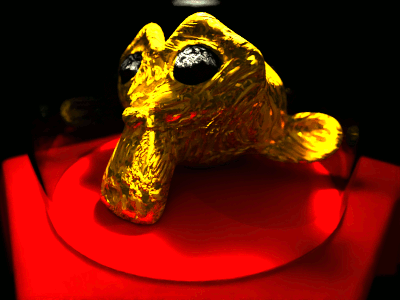
\includegraphics[width=\linewidth]{Medien/suzanne-raw}
				\caption{Raw}
			\end{subfigure}
			\begin{subfigure}{0.33\linewidth}
				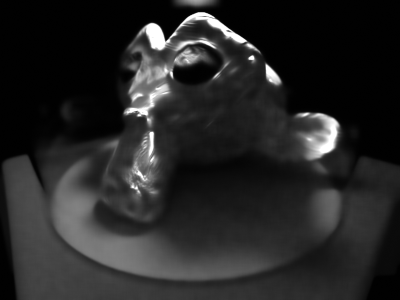
\includegraphics[width=\linewidth]{Medien/suzanne-intensity}
				\caption{Intensität}
			\end{subfigure}
			\begin{subfigure}{0.33\linewidth}
				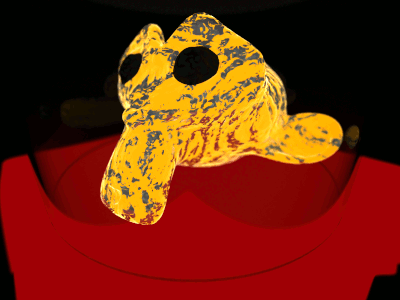
\includegraphics[width=\linewidth]{Medien/suzanne-albedo}
				\caption{Albedo}
			\end{subfigure}
			\begin{subfigure}{0.33\linewidth}
				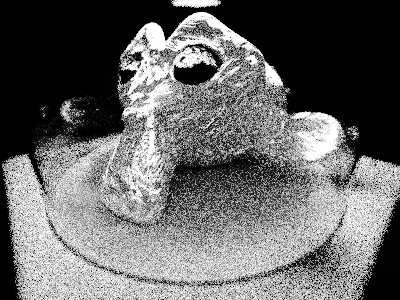
\includegraphics[width=\linewidth]{Medien/suzanne-variance}
				\caption{Varianz}
			\end{subfigure}
			\begin{subfigure}{0.33\linewidth}
				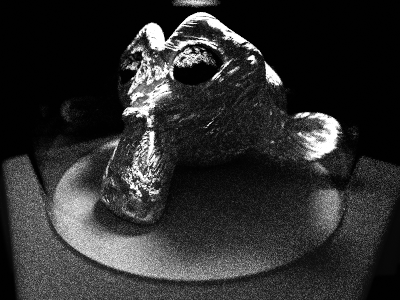
\includegraphics[width=\linewidth]{Medien/suzanne-sw}
				\caption{Schwarz-Weiß}
			\end{subfigure}
			\begin{subfigure}{0.33\linewidth}
				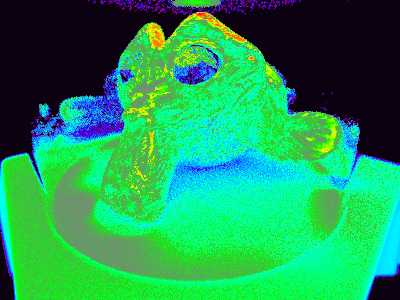
\includegraphics[width=\linewidth]{Medien/suzanne-false-color}
				\caption{Falschfarben}
			\end{subfigure}
			\caption[Suzanne in verschiedenen Renderpasses]{Suzanne, das Maskottchen von Blender mit Goldmaterial in verschiedenen Render-Passes}
			\label{fig:suzanne}
		\end{figure}
		\autoref{fig:suzanne} besteht aus mehreren Teilen, die mit  \lstinline[language=thesis-latexbeispiel]|\begin{subfigure}{0.33\linewidth}| in die \lstinline[language=thesis-latexbeispiel]|figure|-Umgebung aufgenommen werden können. 
		\lstinline[language=thesis-latexbeispiel]|0.33\linewidth| gibt dabei an, dass die Breite der eingefügten Unterabbildung \SI{33}{\percent} der aktuellen Textbreite entsprechen soll.
		
	\section{Tabellen}
		\autoref{tab:beispiel} zeigt eine beispielhafte Tabelle.
		Tabellen werden in der \lstinline[language=thesis-latexbeispiel]|table|-Umgebung gesetzt und sind genau wie Abbildungen \emph{float}-Objekte (siehe \autoref{sec:wissen:float}).
		Die eigentliche Tabelle kann dann \zb{} mit der \lstinline[language=thesis-latexbeispiel]|tabular|-Umgebung gesetzt werden.
		\LaTeX-Editoren wie \emph{TeXstudio} bieten benutzerfreundliche Hilfmittel zur Bearbeitung und automatischen Quelltextformatierung von Tabellen, falls man im Quelltext den Überblick verlieren sollte.
		\begin{table}[bh]
			\centering
			\begin{vorlagenbeispiel}
				\begin{tabular}{l|cr} % lcr: jeder Buchstabe steht für eine Spalte
					(l)eft  & (c)enter & (r)ight \\ % Spalten werden mit & getrennt, Zeilen mit \\ beendet
					\hline                          % \hline erzeugt eine horizontale Linie
					Hier    & steht    & etwas   \\
					in      & einer    & Tabelle
				\end{tabular}
			\end{vorlagenbeispiel}
			\caption{Beispiel zu Tabellen}
			\label{tab:beispiel}
		\end{table}
		\begin{lstlisting}[language=thesis-latexbeispiel]
\begin{table}
	\centering
	\begin{tabular}{l|cr} % lcr: jeder Buchstabe ist eine Spalte
		% Spalten werden mit & getrennt und mit \\ beendet
		(l)eft  & (c)enter & (r)ight \\	
		\hline  % erzeugt eine horizontale Linie
		Hier    & steht    & etwas   \\
		in      & einer    & Tabelle
	\end{tabular}
	\caption{Beispiel zu Tabellen}
	\label{tab:beispiel}
\end{table}
		\end{lstlisting}
		
		
	\section{Quellcode}
		\emph{Für Quellcode nutzt diese Vorlage das Paket \lstinline|listings|.}
		\medskip
		
		Mit \lstinline{\lstinline[language=C]|printf("%d", 42);|} kann Quellcode, z.B. \begin{vorlagenbeispiel}
		\lstinline[language=C]|printf("%d", 42);|
		\end{vorlagenbeispiel} mitten im Text gesetzt werden.
		Der optionale Parameter \lstinline[language=thesis-latexbeispiel]|language=C| gibt dabei an, dass der gezeigte Code in der Programmiersprache \emph{C} vorliegt.
%		
		Die Dokumentation des \lstinline[language=thesis-latexbeispiel]|listings|-Paketes enthält eine vollständige Liste der vordefinierten Programmiersprachen.
		Es gibt ausserdem die Möglichkeit Syntaxhighlighting für weitere Sprachen selber zu definieren.
		\bigskip
		
		Einen abgesetzten Code-Block erzeugt man mit \lstinline[language=thesis-latexbeispiel]|\begin{lstlisting}[language=C]|. Es ist auch möglich Quellcode-Dateien direkt einzubinden (\lstinline[language=thesis-latexbeispiel]|\lstinputlisting{/pfad/zum/quell.code}|), nur einen bestimmten Ausschnitt des Quellcodes anzuzeigen oder die Zeilennummerierung anzupassen (siehe \autoref{code}).
		
		\begin{vorlagenbeispiel}
			\begin{lstlisting}[label=code, language=C, caption={Hello World-Beispiel im lstlisting-Beispiel},firstnumber=1234, emph={printf, schokostuecke}] 
#include <stdio.h>    // Für printf/scanf etc.
#include <stdlib.h>   // Speicherverwaltung & EXIT_SUCCESS/EXIT_FAILURE-Makros

int main(void){
	printf("Hallo LaTeX!\n"); // Textausgabe-Beispiel
	return EXIT_SUCCESS;
}

// In dieser Vorlage sind auch ä,ö,ü,ß und Ä,Ö,Ü erlaubt
			\end{lstlisting}
		\end{vorlagenbeispiel}
		
		Neben \lstinline|language| gibt es noch weitere optionale Parameter, mit denen das Erscheinungsbild angepasst werden kann.
		In \autoref{code} wurden \lstinline|label=labelname| (kann man referenzieren), \lstinline|caption={Beschriftung des Quellcode-Blocks}| und \lstinline|firstnumber=1234| zum Anpassen der Zeilennummerierung verwendet.
	
	\section{Labels \& Referenzen}\label{label-name}
		Überschriften, Abbildungen, Tabellen usw. werden von \LaTeX{} automatisch nummeriert.
%		
		Will man auf einen bestimmten Textabschnitt oder z.B. auf eine Grafik verweisen, so setzt man am Ziel ein \lstinline|\label{labelname}| und referenzenziert dieses dann mit \lstinline|\ref{labelname}|. \lstinline|\autoref{labelname}| ergänzt automatisch den Typ des referenzierten Objekts:
%		
		\begin{vorlagenbeispiel}
		Wenn ich den aktuellen Abschnitt mit \lstinline|ref| referenziere sieht, ergibt sich \ref{label-name} (also nur die Nummer), nutzt man \lstinline|\autoref{labelname}]| ist auch der Typ des Objekts mit dabei: \autoref{label-name}.
%		
		Es ist natürlich auch möglich, \autoref{code} oder \autoref{fig:beispiel} zu referenzieren.
		\end{vorlagenbeispiel}
		
		Mit dem Befehl \lstinline|\nameref{labelname}| erhält man statt der Nummer den Namen des referenzierten Objekts:
		\begin{vorlagenbeispiel}
			Der aktuelle Abschnitt hat die Nummer \ref{label-name} und heißt \enquote{\nameref{label-name}}.
		\end{vorlagenbeispiel}
			
	\section{URLs}
		Mit \lstinline[language=thesis-latexbeispiel]|\url{https://www.blender.org}| lassen sich URLs setzen, die man im PDF dann auch anklicken kann. Der dezente Rahmen um den Link herum wird lediglich angezeigt, beim Drucken aber nicht mit ausgedruckt.
		
		\begin{vorlagenbeispiel}
			Die Open-Source Software Blender (\url{https://www.blender.org}) ist ein mächtiges Allround-Werkzeug für die Erstellung von 3D-Grafik, welches unter anderem die Bereiche Modellierung, Texturierung, Rendering, Rigging, Physik-Simulation, Partikelsimulation, Sculpting, Animation, Videotracking, Videobearbeitung, Compositing und Skripting abdeckt.
		\end{vorlagenbeispiel}
		\medskip

		Will man einen Link absichtlich nur im PDF setzen, die URL aber nicht als Text anzeigen, ist dies mit \lstinline[language=thesis-latexbeispiel]|\href{url}{text}| möglich:
%		
		\begin{vorlagenbeispiel}
			Mit dem sogenannten \href{https://www.blender.org/features/grease-pencil/}{Grease Pencil}-Werkzeug können Künstler 2D Zeichnungen in einer 3D Umgebung erstellen.
			Ursprünglich lediglich ein einfaches Werkzeug für Anmerkungen (daher der Name) wurde es seit \href{https://www.blender.org/download/releases/2-73/}{Blender Version 2.73} zu einem deutlich mächtigeren Werkzeug zur Animation im 2D-Stil weiterentwickelt.
		\end{vorlagenbeispiel}		
		
	\section{Todos}
			Solange die Thesis noch nicht fertig ist, wird man immer mal wieder \enquote{Todos} haben, also Dinge, die noch zu erledigen sind.
			Dank dem \LaTeX-Paket \lstinline[language=thesis-latexbeispiel]|todonotes| kann man diese ganz einfach mit \lstinline[language=thesis-latexbeispiel]|\todo{Hier ist noch etwas zu tun}|\todo{Hier ist noch etwas zu tun} hinzufügen.
	%		
			Mit \lstinline[language=thesis-latexbeispiel]|\listoftodos| lässt sich eine Liste aller Todos im aktuellen Dokument ausgeben.
		
	\section{Glossareinträge \& Symbole}
		\emph{Für Glossareinträge und Symbole nutzt diese Vorlage das Paket \lstinline|glossaries-extra|}
		\medskip
		
		\subsection{Glossar}
			Glossareinträge werden in der Datei \lstinline|Glossar.tex| definiert. Mit \lstinline[language=thesis-latexbeispiel]|\gls{labelname}| können sie im Text verwendet werden:
%			
			\begin{vorlagenbeispiel}
				Es gibt ganz tolle \gls{crc}-Algorithmen, die eine \gls{crc} wirklich genau nach dem Schema typischer \glspl{crc} berechnen.
				Hier ist ein \gls{ex} für einen Glossar-Eintrag. 
				Und hier noch die tolle Abkürzung \gls{svm}, \gls{bspw} stehend für \gls{svm}.
			\end{vorlagenbeispiel}
		\subsection{Symbole}
			Mathematische und physikalische Symbole können ebenfalls in der \lstinline|Glossar.tex| angegeben werden.
			Im Text werden sie mit \lstinline[language=thesis-latexbeispiel]|\glssymbol{labelname}| angesprochen\footnote{Mit \textbackslash gls würde lediglich ihr Name ausgegeben}:
%			
			\begin{vorlagenbeispiel}
				Die ersten drei Buchstaben des griechischen Alphabets sind \glssymbol{alpha}, \glssymbol{beta} und natürlich \glssymbol{gamma}. Die Leere Menge wird mit \glssymbol{emptyset} notiert.
			\end{vorlagenbeispiel}